% !TeX spellcheck = de_AT_frami
\documentclass[10pt,a4paper]{article}
\usepackage[utf8x]{inputenc}
\usepackage{ucs}
\usepackage{amsmath}
\usepackage{amsfonts}
\usepackage{amssymb}
\usepackage{graphicx}
\usepackage{txfonts}
\usepackage[dvipsnames]{xcolor}
\usepackage{geometry}
\usepackage{graphicx}
\usepackage{epstopdf}
\epstopdfsetup{update}
\geometry{margin= 2cm}

\setlength\parindent{0pt}

\begin{document}
	\pagenumbering{gobble}
	\section*{5. Numerik Übungen 2017/18}
	\paragraph{T7}\mbox{}\\
	\textbf{Gegeben sind die Punkte (-2, 71), (-1, 63), (1, 35), (1, 39) und (4, -37).\\
	Erstellen Sie das Differenzentableau und bestimmen Sie das Newtonsche Interpolationspolynom durch die Punkte.} \\
	Allgemeines Differenzenschema für 5 Punkte
   \begin{align*}
   \begin{array}{cc|cccc}
   	x_i & y_i &              \delta y_i              &                     \delta^2 y_i                     &                       \delta^3 y_i                       &                       \delta^4 y_i                       \\ \hline
   	x_0 & y_0 &  \\
   	    &     & \delta y_0 = \frac{y_1-y_0}{x_1-x_0} &  \\
   	x_1 & y_1 &                                      & \delta^2 y_0 = \frac{\delta y_1-\delta y_0}{x_2-x_0} &  \\
   	    &     & \delta y_1 = \frac{y_2-y_1}{x_2-x_1} &                                                      & \delta^3 y_0 = \frac{\delta^2 y_1-\delta^2 y_0}{x_3-x_0} &  \\
   	x_2 & y_2 &                                      & \delta^2 y_1 = \frac{\delta y_2-\delta y_1}{x_3-x_1} &                                                          & \delta^4 y_0 = \frac{\delta^3 y_1-\delta^2 y_0}{x_4-x_0} \\
   	    &     & \delta y_2 = \frac{y_3-y_2}{x_3-x_2} &                                                      & \delta^3 y_1 = \frac{\delta^2 y_2-\delta^2 y_1}{x_4-x_1} &  \\
   	x_3 & y_3 &                                      & \delta^2 y_2 = \frac{\delta y_3-\delta y_2}{x_4-x_2} &  \\
   	    &     & \delta y_3 = \frac{y_4-y_3}{x_4-x_3} &  \\
   	x_4 & y_4 &
   \end{array}
   \end{align*}
   Mit den Punkten
   \begin{align*}
   	\begin{array}{rr}
	   	x_i & y_i \\
   		-2 & 71  \\
   		-1 & 63  \\
   		1  & 35  \\
   		2  & 39  \\
   		4  & -37
   	\end{array}
   \end{align*}
ergibt sich
\begin{align*}
\begin{array}{cc|cccc}
	x_i & y_i &              \delta y_i               &              \delta^2 y_i              &             \delta^3 y_i              &             \delta^4 y_i             \\ \hline
	-2  & 71  &  \\
	    &     & \delta y_0 = \frac{63-71}{-1+2} = -8  &  \\
	-1  & 63  &                                       & \delta^2 y_0 = \frac{-14+8}{1+2} = -2  &  \\
	    &     & \delta y_1 = \frac{35-63}{1+1} = -14  &                                        &  \delta^3 y_0 = \frac{6+2}{2+2} = 2   &  \\
	 1  & 35  &                                       &  \delta^2 y_1 = \frac{4+14}{2+1} = 6   &                                       & \delta^4 y_0 = \frac{-4-2}{4+2} = -1 \\
	    &     &  \delta y_2 = \frac{39-35}{2-1} = 4   &                                        & \delta^3 y_1 = \frac{-14-6}{4+1} = -4 &  \\
	 2  & 39  &                                       & \delta^2 y_2 = \frac{-38-4}{4-1} = -14 &                                       &  \\
	    &     & \delta y_3 = \frac{-37-39}{4-2} = -38 &  \\
	 4  & -37 &                                       &
\end{array}
\end{align*}
kürzer
\begin{align*}
\begin{array}{cc|cccc}
	x_i & y_i &    \delta y_i    &    \delta^2 y_i    &   \delta^3 y_i    &   \delta^4 y_i    \\ \hline
	-2  & 71  &  \\
	    &     & \delta y_0 = -8  &  \\
	-1  & 63  &                  & \delta^2 y_0 = -2  &  \\
	    &     & \delta y_1 = -14 &                    & \delta^3 y_0 = 2  &  \\
	 1  & 35  &                  &  \delta^2 y_1 = 6  &                   & \delta^4 y_0 = -1 \\
	    &     &  \delta y_2 = 4  &                    & \delta^3 y_1 = -4 &  \\
	 2  & 39  &                  & \delta^2 y_2 = -14 &                   &  \\
	    &     & \delta y_3 = -38 &  \\
	 4  & -37 &                  &
\end{array}
\end{align*}
Das Interpolationspolynom lautet allgemein für n+1 Punkte nach Newton
\begin{align*}
p(x) = y_0 + (x-x_0)\delta y_0 + (x-x_0)(x-x_1)\delta^2 y_0 + \cdots + (x-x_0)(x-x_1)\cdots(x-x_{n-1})\delta^n y_0.
\end{align*}
Mit obigen Differenzenschema ergibt sich
\begin{align*}
	p(x) & = 71 + (x+2)(-8) + (x+2)(x+1)(-2) + (x+2)(x+1)(x-1)2 + (x+2)(x+1)(x-1)(x-2)(-1) \\
	     & = 71 + (x+2)(-8) + (x^2+3x+2)(-2) + (x^3+2x^2-x-2)2 + (x^4-5x^2+4)(-1)          \\
	     & = 71 -8x - 16 - 2x^2 - 6x - 4 + 2x^3 + 4x^2 - 2x - 4 -x^4 + 5x^2 - 4            \\
	     & = -x^4 + 2x^3 + 7x^2 - 16x + 43                                                 \\
	     & = (-x^3 + 2x^2 + 7x - 16)x + 43                                                 \\
	     & = ((-x^2 + 2x + 7)x - 16)x + 43                                                 \\
	     & = (((-x + 2)x + 7)x - 16)x + 43                                                 \\
	p(x) & = ((((-1)x + 2)x + 7)x - 16)x + 43
\end{align*}
\begin{figure}[htbp]
	\centering
	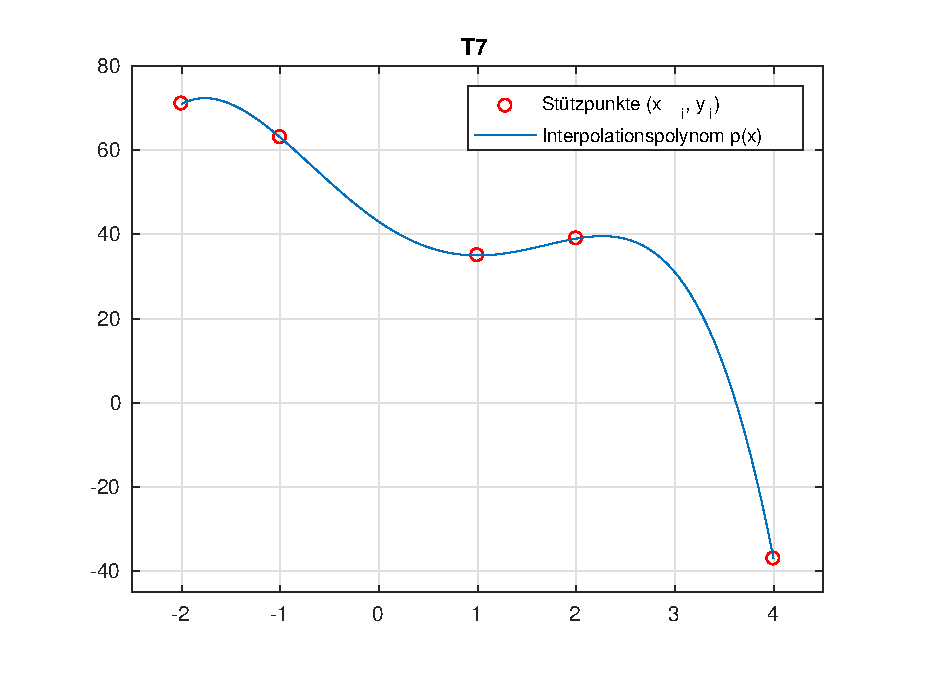
\includegraphics[width=0.7\textwidth]{T7}
	\caption{Punkte $(x_1, y_i)$ und Interpolationspolynom $p(x)$}
\end{figure}

\newpage

\paragraph{T8}\mbox{}\\
\textbf{Werten Sie das Newtonsche Interpolationspolynom aus Aufgabe (T7) mit Hilfe des Horner-Schemas für Newtonsche Interpolationspolynome an den Stellen $\mathbf{x=2}$ und $\mathbf{x=3}$ aus.}

Allgemein nach Herausheben der Faktoren $(x-x_i)$ beim Newtonschen Interpolationspolynom
\begin{align*}
	p(x)=y_0+(x-x_0)(\delta y_0+ (x-x_1)(\delta^2y_0+\dots+(x-x_{n-2})(\delta^{n-1}y_0+(x-x_{n-1})\delta^n y_0)\dots)).
\end{align*}
Für unser Beispiel gilt somit
\begin{align*}
p(x) & = 71 + {\color{red}(x+2)}(-8) + {\color{red}(x+2)}{\color{orange}(x+1)}(-2) + {\color{red}(x+2)}{\color{orange}(x+1)}{\color{cyan}(x-1)}\cdot 2 + {\color{red}(x+2)}{\color{orange}(x+1)}{\color{cyan}(x-1)}{\color{green}(x-2)}(-1) \\
& = 71 + {\color{red}(x+2)}(-8 + {\color{orange}(x+1)}(-2 + {\color{cyan}(x-1)}(2 + {\color{green}(x-2)}(-1)))) 
\end{align*}
Das Schema für die Rechnung per Hand lautet allgemein
\begin{align*}
p(x) = \delta^0 y_0 + (x-x_0)\delta^1 y_0 + (x-x_0)(x-x_1)\delta^2 y_0 + \cdots + (x-x_0)(x-x_1)\cdots(x-x_{n-1})\delta^n y_0.
\end{align*}
\begin{align*}
\begin{array}[htbp]{c|cccccc}
	  & \delta^n y_0 & \delta^{n-1} y_0     & \delta^{n-2} y_0         & \cdots & \delta^1 y_0     & \delta^0 y_0     \\
	x & 0            & (x-x_{n-1})\cdot b_n & (x-x_{n-2})\cdot b_{n-1} & \cdots & (x-x_1)\cdot b_2 & (x-x_0)\cdot b_1 \\ \hline
	  & b_n          & b_{n-1}              & b_{n-2}                  & \cdots & b_1              & b_0=p(x)
\end{array}
\end{align*}
Angewendet für $x=2$ und 
\begin{align*}
	p(x) = {\color{Fuchsia}71} + (x+2){\color{SpringGreen}(-8)} + (x+2)(x+1){\color{Apricot}(-2)} + (x+2)(x+1)(x-1)\cdot{\color{Turquoise}2} + {\color{red}(x+2)}{\color{orange}(x+1)}{\color{cyan}(x-1)}{\color{green}(x-2)}{\color{Lavender}(-1)}
\end{align*}
(vgl. Bsp.3.4 S.45)
\begin{align*}
&\begin{array}[htbp]{c|rrrrr}
	      & {\color{Lavender}-1} & {\color{Turquoise}2}                                        & {\color{Apricot}-2}                                                   & {\color{SpringGreen}-8}                      & {\color{Fuchsia}71} \qquad \quad \\
	x = 2 & \downarrow           & {\color{red}-1}\cdot{\color{green}({\color{black}2}-2)} = 0 & {\color{CarnationPink}2} \cdot {\color{cyan}({\color{black}2}-1)} = 2 & 0 \cdot {\color{orange}({\color{black}2}+1)} = 0 & -8 \cdot {\color{red}({\color{black}2}+2)} = -32 \qquad \quad \\ \hline
	      & {\color{red}-1}      & {\color{Turquoise}2}+0={\color{CarnationPink}2}             & {\color{Apricot}-2}+ 2 = 0                                            & {\color{SpringGreen}-8} + 0 = -8                                          & {\color{Fuchsia}71}-32 = 39 = p(2)
\end{array} \\
&\begin{array}[htbp]{c|rrrrr}
	      & {\color{Lavender}-1} & {\color{Turquoise}2}     & {\color{Apricot}-2} & {\color{SpringGreen}-8} & {\color{Fuchsia}71} \qquad \quad \\
	x = 2 & \downarrow           & 0                        & 2                   & 0                       & -32 \qquad \quad                 \\ \hline
	      & {\color{red}-1}      & {\color{CarnationPink}2} & 0                   & -8                      & 39 = p(2)
\end{array}
\end{align*}



Alternativ für $x=2$ und $p(x) = -x^4 + 2x^3 + 7x^2 - 16x + 43$ geschrieben (vgl. Bsp.3.3 S.45)
\begin{align*}
&\begin{array}[htbp]{c|rrrrr}
	      & {\color{Lavender}-1} & {\color{Turquoise}2}                    & 7      & -16         & 43 \qquad \quad \\
	x = 2 & \downarrow           & {\color{red}-1}*{\color{Turquoise}2}=-2 & 0*2= 0 & 7*2 = 14    & -2*2 = -4 \qquad \quad \\ \hline
	      & {\color{red}-1}      & 2+(-2)=0                                & 0*7=7  & -16+14 = -2 & 43+(-4) = 39 = p(2)
\end{array} \\
&\begin{array}[htbp]{c|rrrrr}
	      & -1         & 2  & 7 & -16 & 43  \qquad \quad      \\
	x = 2 & \downarrow & -2 & 0 & 14  & -4 \qquad \quad      \\ \hline
	      & -1         & 0  & 7 & -2  & 39 = p(2)
\end{array}
\end{align*}
mit $x=3$
\begin{align*}
&\begin{array}[htbp]{c|rrrrr}
	      & -1         & 2       & 7       & -16        & 43         \qquad \quad \\
	x = 3 & \downarrow & -1*3=-3 & -1*3=-3 & 4*3 = 12   & -4*3 = -12 \qquad \quad \\ \hline
	      & -1         & -3+2=-1 & -3+7=4  & 12-16 = -4 & -12+43 = 31 = p(3)
\end{array} \\
&\begin{array}[htbp]{c|rrrrr}
	      & -1         & 2  & 7  & -16 & 43   \qquad \quad \\
	x = 2 & \downarrow & -3 & -3 & 12  & -12  \qquad \quad \\ \hline
	      & -1         & -1 & 4  & -4  & 31 = p(3)
\end{array}
\end{align*}
\end{document}